\section{Sonar}

% Throughout this thesis only one type of sonar is considered, the mechanical
% imaging active sonar (section \ref{ss:avaible_models}). Sonars have a common
% underlying principle of operation, but vary greatly on aplication and hardware constituition.

Throughout this thesis one specific type of sonar will be considered, the
mechanical imaging active sonar (section \ref{ss:avaible_models}). Sonars have a common
underlying principle of operation, but vary greatly on application and hardware
constitution.


Sonars are, in some sense, the acoustic analog of a camera. They use sound,
instead of light, to capture information about the environment. Hence, to better
understand \textit{how} they operate and \textit{what} they are used for, it is
important to have a clear concept of sound.

\subsection{Physics of Sound}

The phenomenon that humans perceive as sound is a pressure wave which
amplitude excesses the medium's mean pressure \cite{FEYNMAN}. It can be
referred to as \textit{compressional} or \textit{longitudinal} waves, contrasting with
\textit{transversal waves}. The difference between these two kinds of waves
%% SrJ?: "particles" ?
relies on the direction of the movement of the particles, being parallel or
perpendicular to the propagation of the wave, respectively\cite{BRUNEAU}.

On the particular, but common, condition of low energy
phenomena\cite{Lefebvre} (with some other suitable requirements\footnote{A
perfect simple fluid in an initial state of stationary homogeneous equilibrium})
the pressure perturbation wave can be described as the \textit{D'Alembert
equation}:
 
\begin{equation}\label{eq:lambert}
\nabla^2 \Phi - \frac{1}{c^2_0}\frac{\partial^2}{\partial t^2} \Phi = 0
\end{equation}

Where $\Phi$ is the velocity potential, a scalar field that helps describing the
sound propagation. Its relation to sound pressure is:

\[ p =  -\rho \frac{\partial}{\partial t}\Phi \]

Which can be directly described as:

\begin{equation} \label{eq:wave}
\nabla^2 p - \frac{1}{c^2_0}\frac{\partial^2}{\partial t^2} p = 0
\end{equation} 
 
Where $p$ is the pressure deviation from the mediums, $\rho$ the density, $c_0$
is the local sound speed and $\nabla^2$ stands for the Laplace operator. These equations are
only valid in free space (no source), however discrete variations of the medium
are treated as boundary conditions, giving origin to reflection and refraction.

Besides pressure, sound has another important derived property: intensity. Much
as the case of electromagnetic waves, sound intensity (or acoustic intensity)
measures the mean value of the sound energy flux (i.e. energy rate
per area):

\begin{equation}\label{eq:intensity_mean}
\vec{I} = \overline{p\vec{v}}
\end{equation}

Where $\vec{I}$ represents the \textit{acoustic intensity} vector, $\vec{v}$ the
\textit{acoustic velocity} (i.e. the velocity of a particle in the medium) and
overline the mean over some time period. The \textit{acoustic
velocity} can also be derived from the velocity potential $\Phi$ as:

\[ \vec{v} = \nabla \Phi\]

When considering a wave far from its source, solutions to the equation
\ref{eq:wave} give rise to a \textit{plane wave}( where the coherent wave front
propagate in a plane). It makes clear the relationship between $\vec{v}$ and
$p$:

\[ \vec{v} = \frac{p}{\rho c_0} \vec{n_0} \]

Where $\vec{n_0}$ is the unit normal vector to the wavefront. Plugging it back to
equation \ref{eq:intensity_mean}:

\begin{equation}\label{eq:intensity_pressure}
\vec{I} = \tfrac{1}{\rho c_0} \overline{p^2} \vec{n_0}
\end{equation}

This equation shows the proportionality between the \textit{acoustic
intensity} and the mean of the square of the pressure. The inverse of the
proportionality constant $\rho c_0$ is called the \textit{characteristic
impedance} because it measures the degree of ``resistance to propagation'' of
the medium.

%By means of the same reasoning about the physical properties

 %(perpendicular to the direction of propagation)

Because the acoustic intensity (and related quantities) varies in orders of
magnitude while propagating, it is common to quantify it on a logarithmic scale,
specifically \textit{decibels} (dB)\cite{LURTON}:

\begin{equation}\label{eq:dB}
I_{dB} = 10~\log_{10}\left(\frac{I}{I_0}\right)
\end{equation} 

Here $I_{dB}$ is the intensity measured in \textit{decibels}, $I$ is the
intensity value and $I_0$ a reference intensity values, usually defined somewhere near the
source. In the case of reflected/refracted wave, $I_0$ may also refers to
the intensity of the incoming wave. A direct relation between the magnitude of
intensity and pressure is found by applying equation \ref{eq:intensity_pressure}
on equation\ref{eq:dB}:

\begin{equation}\label{eq:dB2}
I_{dB} = 20~\log_{10}\left(\frac{p_{\text{rms}}}{p_0}\right)
\end{equation}

Where $p_{\text{rms}}$ is the \textit{rms} (Root mean squared) value of the
wave's pressure ({\small $\sqrt{\text{\tiny \(\overline{p^2}\)}}$}) and $p_0$ is
a pressure value of reference, for underwater acoustics this value is the
micro Pascal (\(p_0 = 1~\mu\text{Pa} \))\cite{LURTON}.


\subsection{Sonar Principle of Operation}

The name Sonar (\textit{\underline{So}und \underline{N}avigation \underline{A}nd
\underline{R}anging}) was originally conceived for any technique that uses
acoustic waves on water for navigation, communication and detection, but
nowadays it is also used for the equipment that generate/receive these
sound waves.

%% SrJ?: cute, but doubtful ...
The history of sonar is considered as having began on the year of 1490 through
the statement of Leonardo Da Vinci aforementioned on the epigraph 
of this chapter\cite{fahy1998fundamentals}. That was the birth of
\textit{passive sonar}'s technology, where the objective is to listen (receive
and process sound waves) the noise from ships, animals and other objects in an attempt detect and
recognize its origin. 

However, as it is not expected that all surfaces emit noise, this passive type
of sonar is not suitable for mapping.
For that purpose, another type of sonar that could probe the surrounds had to be
devised, those would be called \textit{active sonars}.

%% SrJ: no transition. Mention both in the subsection introduction and then go
% on

\subsubsection{Active Sonar}

The concept of an \textit{active sonar}, one that emits a sound wave and detects
its return (as in figure \ref{fig:sonar_principle}), is much recent. The
loss of the \textit{HMS Titanic} due to a collision with an iceberg during its
first voyage on April 15 of 1912 \cite{histsonar} fostered the development of a sonar
to detect objects kilometers away. Also, during World War I,
Allied shipping losses to U-boat attacks further stimulated advances on
techniques for uncovering of submerged enemies.

\begin{figure}
	\centering
		\begin{tikzpicture}[thick,scale=0.3, every node/.style={transform shape},line
	cap=round,line join=round,>=triangle 45,x=1.0cm,y=1.0cm] \clip(2.4174670085420336,-13.987437987397216) rectangle (50.355233369869445,8.357537118695749);
	\fill[color=ffqqqq,fill=ffqqqq,fill opacity=0.1] (5.,-4.) -- (5.,-1.) -- (8.,-1.) -- (10.,0.) -- (10.,-5.) -- (8.,-4.) -- cycle;
	\draw [color=qqqqff,fill=qqqqff,fill opacity=0.53] (46.,-2.5) circle (1.7879362227931317cm);
	\draw [color=ffqqqq] (5.,-4.)-- (5.,-1.);
	\draw [color=ffqqqq] (5.,-1.)-- (8.,-1.);
	\draw [color=ffqqqq] (8.,-1.)-- (10.,0.);
	\draw [color=ffqqqq] (10.,0.)-- (10.,-5.);
	\draw [color=ffqqqq] (10.,-5.)-- (8.,-4.);
	\draw [color=ffqqqq] (8.,-4.)-- (5.,-4.);
	\draw [shift={(5.,-2.5)},color=ffqqqq]  plot[domain=-0.46364760900080615:0.4636476090008061,variable=\t]({1.*8.375892603043697*cos(\t r)+0.*8.375892603043697*sin(\t r)},{0.*8.375892603043697*cos(\t r)+1.*8.375892603043697*sin(\t r)});
	\draw [color=ffffff] (4.,2.)-- (50.,2.);
	\draw [color=ffffff] (50.,2.)-- (50.,10.);
	\draw [color=ffffff] (50.,10.)-- (4.,10.);
	\draw [color=ffffff] (4.,10.)-- (4.,2.);
	\draw [color=ffffff] (44.,-8.)-- (4.,-8.);
	\draw [color=ffffff] (4.,-8.)-- (4.,-16.);
	\draw [color=ffffff] (4.,-16.)-- (42.20321483552447,-16.390821937761867);
	\draw [color=ffffff] (42.20321483552447,-16.390821937761867)-- (44.,-8.);
	\draw [shift={(46.,-2.5)},dash pattern=on 3pt off 3pt,color=qqqqff]  plot[domain=2.6779450445889874:3.6052402625905975,variable=\t]({1.*2.785722659294224*cos(\t r)+0.*2.785722659294224*sin(\t r)},{0.*2.785722659294224*cos(\t r)+1.*2.785722659294224*sin(\t r)});
	\draw [shift={(46.,-2.5)},dash pattern=on 3pt off 3pt,color=qqqqff]  plot[domain=2.6779450445889874:3.6052402625905993,variable=\t]({1.*5.571445318588448*cos(\t r)+0.*5.571445318588448*sin(\t r)},{0.*5.571445318588448*cos(\t r)+1.*5.571445318588448*sin(\t r)});
	\draw [shift={(46.,-2.5)},dash pattern=on 3pt off 3pt,color=qqqqff]  plot[domain=2.677945044588987:3.6052402625905997,variable=\t]({1.*8.357167977882664*cos(\t r)+0.*8.357167977882664*sin(\t r)},{0.*8.357167977882664*cos(\t r)+1.*8.357167977882664*sin(\t r)});
	\draw [shift={(46.,-2.5)},dash pattern=on 3pt off 3pt,color=qqqqff]  plot[domain=2.677945044588987:3.6052402625905993,variable=\t]({1.*11.142890637176889*cos(\t r)+0.*11.142890637176889*sin(\t r)},{0.*11.142890637176889*cos(\t r)+1.*11.142890637176889*sin(\t r)});
	\draw [shift={(46.,-2.5)},dash pattern=on 3pt off 3pt,color=qqqqff]  plot[domain=2.677945044588987:3.605240262590599,variable=\t]({1.*13.928613296471113*cos(\t r)+0.*13.928613296471113*sin(\t r)},{0.*13.928613296471113*cos(\t r)+1.*13.928613296471113*sin(\t r)});
	\draw [shift={(46.,-2.5)},dash pattern=on 3pt off 3pt,color=qqqqff]  plot[domain=2.677945044588987:3.6052402625905993,variable=\t]({1.*16.714335955765335*cos(\t r)+0.*16.714335955765335*sin(\t r)},{0.*16.714335955765335*cos(\t r)+1.*16.714335955765335*sin(\t r)});
	\draw [shift={(46.,-2.5)},dash pattern=on 3pt off 3pt,color=qqqqff]  plot[domain=2.677945044588987:3.6052402625905993,variable=\t]({1.*19.500058615059555*cos(\t r)+0.*19.500058615059555*sin(\t r)},{0.*19.500058615059555*cos(\t r)+1.*19.500058615059555*sin(\t r)});
	\draw [shift={(46.,-2.5)},dash pattern=on 3pt off 3pt,color=qqqqff]  plot[domain=2.677945044588987:3.6052402625905993,variable=\t]({1.*22.285781274353777*cos(\t r)+0.*22.285781274353777*sin(\t r)},{0.*22.285781274353777*cos(\t r)+1.*22.285781274353777*sin(\t r)});
	\draw [shift={(46.,-2.5)},dash pattern=on 3pt off 3pt,color=qqqqff]  plot[domain=2.677945044588987:3.605240262590599,variable=\t]({1.*25.071503933648003*cos(\t r)+0.*25.071503933648003*sin(\t r)},{0.*25.071503933648003*cos(\t r)+1.*25.071503933648003*sin(\t r)});
	\draw [shift={(46.,-2.5)},dash pattern=on 3pt off 3pt,color=qqqqff]  plot[domain=2.677945044588987:3.6052402625905993,variable=\t]({1.*27.857226592942222*cos(\t r)+0.*27.857226592942222*sin(\t r)},{0.*27.857226592942222*cos(\t r)+1.*27.857226592942222*sin(\t r)});
	\draw [shift={(5.,-2.5)},color=ffqqqq]  plot[domain=-0.46364760900080615:0.4636476090008061,variable=\t]({1.*11.16161526233792*cos(\t r)+0.*11.16161526233792*sin(\t r)},{0.*11.16161526233792*cos(\t r)+1.*11.16161526233792*sin(\t r)});
	\draw [shift={(5.,-2.5)},color=ffqqqq]  plot[domain=-0.46364760900080615:0.4636476090008061,variable=\t]({1.*13.947337921632139*cos(\t r)+0.*13.947337921632139*sin(\t r)},{0.*13.947337921632139*cos(\t r)+1.*13.947337921632139*sin(\t r)});
	\draw [shift={(5.,-2.5)},color=ffqqqq]  plot[domain=-0.46364760900080615:0.4636476090008061,variable=\t]({1.*16.733060580926363*cos(\t r)+0.*16.733060580926363*sin(\t r)},{0.*16.733060580926363*cos(\t r)+1.*16.733060580926363*sin(\t r)});
	\draw [shift={(5.,-2.5)},color=ffqqqq]  plot[domain=-0.46364760900080615:0.4636476090008061,variable=\t]({1.*19.51878324022059*cos(\t r)+0.*19.51878324022059*sin(\t r)},{0.*19.51878324022059*cos(\t r)+1.*19.51878324022059*sin(\t r)});
	\draw [shift={(5.,-2.5)},color=ffqqqq]  plot[domain=-0.46364760900080615:0.4636476090008061,variable=\t]({1.*22.304505899514808*cos(\t r)+0.*22.304505899514808*sin(\t r)},{0.*22.304505899514808*cos(\t r)+1.*22.304505899514808*sin(\t r)});
	\draw [shift={(5.,-2.5)},color=ffqqqq]  plot[domain=-0.46364760900080615:0.4636476090008061,variable=\t]({1.*25.090228558809027*cos(\t r)+0.*25.090228558809027*sin(\t r)},{0.*25.090228558809027*cos(\t r)+1.*25.090228558809027*sin(\t r)});
	\draw [shift={(5.,-2.5)},color=ffqqqq]  plot[domain=-0.46364760900080615:0.4636476090008061,variable=\t]({1.*27.875951218103253*cos(\t r)+0.*27.875951218103253*sin(\t r)},{0.*27.875951218103253*cos(\t r)+1.*27.875951218103253*sin(\t r)});
	\draw [shift={(5.,-2.5)},color=ffqqqq]  plot[domain=-0.46364760900080615:0.4636476090008061,variable=\t]({1.*30.661673877397476*cos(\t r)+0.*30.661673877397476*sin(\t r)},{0.*30.661673877397476*cos(\t r)+1.*30.661673877397476*sin(\t r)});
	\draw [shift={(5.,-2.5)},color=ffqqqq]  plot[domain=-0.46364760900080615:0.4636476090008061,variable=\t]({1.*33.4473965366917*cos(\t r)+0.*33.4473965366917*sin(\t r)},{0.*33.4473965366917*cos(\t r)+1.*33.4473965366917*sin(\t r)});
	\draw [shift={(5.,-2.5)},color=ffqqqq]  plot[domain=-0.46364760900080615:0.4636476090008061,variable=\t]({1.*36.23311919598592*cos(\t r)+0.*36.23311919598592*sin(\t r)},{0.*36.23311919598592*cos(\t r)+1.*36.23311919598592*sin(\t r)});
	\draw [shift={(5.,-2.5)},color=ffqqqq]  plot[domain=-0.46364760900080615:0.4636476090008061,variable=\t]({1.*39.018841855280144*cos(\t r)+0.*39.018841855280144*sin(\t r)},{0.*39.018841855280144*cos(\t r)+1.*39.018841855280144*sin(\t r)});
	\draw [color=ffqqqq] (24.,5.5)-- (27.,5.5);
	\draw [color=ffqqqq] (27.,5.5)-- (27.,5.);
	\draw [color=ffqqqq] (27.,5.)-- (27.5,5.5);
	\draw [color=ffqqqq] (27.5,5.5)-- (28.,6.);
	\draw [color=ffqqqq] (28.,6.)-- (27.5,6.5);
	\draw [color=ffqqqq] (27.5,6.5)-- (27.,7.);
	\draw [color=ffqqqq] (27.,7.)-- (27.,6.5);
	\draw [color=ffqqqq] (27.,6.5)-- (22.,6.5);
	\draw [color=ffqqqq] (22.,6.5)-- (22.,5.5);
	\draw [color=ffqqqq] (22.,5.5)-- (24.,5.5);
	\draw [color=xdxdff] (26.,-12.)-- (23.,-12.);
	\draw [color=xdxdff] (23.,-12.)-- (23.,-12.5);
	\draw [color=xdxdff] (23.,-12.5)-- (22.5,-12.);
	\draw [color=xdxdff] (22.5,-12.)-- (22.,-11.5);
	\draw [color=xdxdff] (22.,-11.5)-- (22.5,-11.);
	\draw [color=xdxdff] (22.5,-11.)-- (23.,-10.5);
	\draw [color=xdxdff] (23.,-10.5)-- (23.,-11.);
	\draw [color=xdxdff] (23.,-11.)-- (28.,-11.);
	\draw [color=xdxdff] (28.,-11.)-- (28.,-12.);
	\draw [color=xdxdff] (28.,-12.)-- (26.,-12.);
	\fill[color=ffffff,fill=ffffff,fill opacity=1.0] (4.,2.) -- (50.,2.) -- (50.,10.) -- (4.,10.) -- cycle;
	\fill[color=ffffff,fill=ffffff,fill opacity=1.0] (44.,-8.) -- (4.,-8.) -- (4.,-16.) -- (42.20321483552447,-16.390821937761867) -- cycle;
	\fill[color=ffqqqq,fill=ffqqqq,fill opacity=1.0] (24.,5.5) -- (27.,5.5) -- (27.,5.) -- (27.5,5.5) -- (28.,6.) -- (27.5,6.5) -- (27.,7.) -- (27.,6.5) -- (22.,6.5) -- (22.,5.5) -- cycle;
	\fill[color=xdxdff,fill=xdxdff,fill opacity=1.0] (26.,-12.) -- (23.,-12.) -- (23.,-12.5) -- (22.5,-12.) -- (22.,-11.5) -- (22.5,-11.) -- (23.,-10.5) -- (23.,-11.) -- (28.,-11.) -- (28.,-12.) -- cycle;
	\draw [color=ffqqqq](22.911186909624416,4.005463478846246) node[anchor=north
	west] {\LARGE\textbf{Outgoing Wave}}; \draw
	[color=qqqqff](23.17101220155573,-9.115713763685088) node[anchor=north west]
	{\LARGE\textbf{Incoming Wave}};
	\end{tikzpicture}

	\caption{Depiction of the working principle of an \textit{active sonar}. The
	red speaker-like object represents the transducer, responsible for
	emitting and receiving the acoustic wave.}
	\label{fig:sonar_principle}
\end{figure}

Active sonars are ranging sensor and the way they infer distance is by measuring
the time between the emission and reception of an acoustic pulse (a time bounded
sound wave) like on \ref{fig:sonar_principle}. Given the mean sound speed of the
medium throughout the path traveled by the pulse, one can infer range\cite{LURTON}:

\begin{equation}
R = \frac{c_0 \Delta t}{2}
\label{eq:delaytodistance}
\end{equation}


Where $R$ is the distance between the source and the target, $c_0$ is the mean
sound speed, $\Delta t$ is the delay between pulse emission and reception, and
the denominator $2$ is a consequence of time measuring the two way
trip of the pulse. When the medium cannot be considered homogeneous, as in long distance travels in
the ocean, additional effects must be taken into account~\cite{Etter2013}.

Active sonars outputs is influenced by various factors, some considered to be
more relevant will be further explored in this section: multipaths, spatial
resolution, bearing indistinguishability and propagation loss compensation
(TVG).

% When the sound wave travels long distances in the ocean,
% sound speed may vary greatly, so, special care should be
% taken\cite{Etter2013}.stratify the environment by same sound speed layers

%% SrJ: no transition ....

\subsubsection{Multipath}

%% SeJ: while theoretically water surface or obstacles do have some refraction
%% Sej: involved, nobody would ever say that at the frequencies sonar work on
%%
%% SeJ: the main source of refraction are the interfaces between water speed
%% SeJ: zones

Besides sound speed variation, another common issue is \textit{multipath}. The
moment a sound wave encounters an interface (e.g. an obstacle like the sea floor
or the water surface), it does not fully bounce back to the source, it also undergoes
reflection in other directions. Thus, an echo that has traveled a longer
path may also arrive, causing a naive application of equation \ref{eq:delaytodistance} to
predict the presence of an object further away (figure \ref{fig:multipath}). For
low-frequency stable signals, the contribution of all multipaths creates an
interference pattern\cite{LURTON}, a fact that will not be further explored. 

\begin{figure}
	\centering
	\begin{tikzpicture}[thick,scale=0.25,line
cap=round,line join=round,>=triangle 45,x=1.0cm,y=1.0cm] \clip(1.6275066818196025,-8.839384430530606) rectangle (51.76470824776055,15.208548396032874);
\clip(3.1041672991448848,-7.273988531661666) rectangle (49.67584843845491,14.87093936751221);
\begin{scriptsize}
\draw [color=xdxdff] (44.21347454534831,-2.428987771071691)-- ++(-2.5pt,-2.5pt) -- ++(5.0pt,5.0pt) ++(-5.0pt,0) -- ++(5.0pt,-5.0pt);
\draw[color=xdxdff] (43.541104898818894,-3.402366846586503) node {$T$};
\draw [color=dcrutc] (42.93049589992042,11.940544124335187)-- ++(-2.0pt,-2.0pt) -- ++(4.0pt,4.0pt) ++(-4.0pt,0) -- ++(4.0pt,-4.0pt);
\draw[color=dcrutc] (42.45630268754179,10.625247954410463) node {$S$};
\draw[color=dcrutc] (-15.15043542855254,31.53574575109661) node {$s$};
\draw[color=xdxdff] (-14.477109918104684,30.37612959421419) node {$r$};
\end{scriptsize}
\fill[color=ffqqqq,fill=ffqqqq,fill opacity=0.1] (5.,-4.) -- (5.,-1.) -- (8.,-1.) -- (10.,0.) -- (10.,-5.) -- (8.,-4.) -- cycle;
\draw [dotted,color=dcrutc] (5.,-2.5) circle (40.586350338762315cm);
\draw [dash pattern=on 3pt off 3pt,color=dcrutc] (44.59640537748493,12.574773620869905) circle (1.7825571147199057cm);
\draw [dotted,color=xdxdff] (5.,-2.5) circle (39.21353884381436cm);
\draw [color=ffqqqq] (5.,-4.)-- (5.,-1.);
\draw [color=ffqqqq] (5.,-1.)-- (8.,-1.);
\draw [color=ffqqqq] (8.,-1.)-- (10.,0.);
\draw [color=ffqqqq] (10.,0.)-- (10.,-5.);
\draw [color=ffqqqq] (10.,-5.)-- (8.,-4.);
\draw [color=ffqqqq] (8.,-4.)-- (5.,-4.);
\draw [color=qqqqff,fill=qqqqff,fill opacity=0.53] (46.,-2.5) circle (1.7879362227931317cm);
\draw [->,line width=1.6pt,dash pattern=on 6pt off 6pt,color=dcrutc] (24.7,5.) -- (42.93049589992042,11.940544124335187);
\draw [->] (10.,-0.5964467005076142) -- (24.7,5.);
\draw [->] (24.7,5.) -- (44.21347454534831,-2.428987771071691);
\draw [->] (44.21347454534831,-2.428987771071691) -- (10.,-2.4909454301421077);
\draw [line width=2.pt] (20.,5.)-- (35.,5.);
\end{tikzpicture}
	\caption{Visualization of a multipath for a high frequency short pulse (much
	smaller than delay times). Black vectors show the path taken by the sound
	wave. Red dashed vector shows the calculated distance by equation
	\ref{eq:delaytodistance}.}
	\label{fig:multipath}
\end{figure}

\subsubsection{Sonar Resolution and CHIRP Pulses}

The minimum distance (or echo delay) that can be resolved by the sonar, depends
on the type of pulse emitted (figure \ref{fig:chirpresolution}). There are two
main types of pulse:
\textit{single frequency} and \textit{chirp}\cite{chirp,gaussianchirp}. Some
sonars use dual frequency to overcome the trade-off between reach and
resolution, given that low-frequency has a longer range and high-frequency a better resolution.

For single frequency sonar, the limit resolution ($\delta R$) depends directly
on the pulse length ($\Delta\text{L}$):

\[ \delta R = \frac{c_0~\Delta\text{L}}{2} \] 

However, that limitation can be overcome by the use of pulse compression (a
cross-correlation filter like matched filters). In this case, a linear varying
frequency signal (chirp), or similar multifrequency systems, has its resolution
related to the bandwidth ($\Delta \text{BW}$):

\[ \delta R = \frac{c_0}{2~\Delta \text{BW}} \]

\begin{figure}
	\centering
	% Need GNUPLOT installed
% also include the command:
% pdflatex --shell-escape --enable-write18
\begin{tikzpicture}[thick,scale=0.25, line
cap=round,line join=round,>=triangle 45,x=1.0cm,y=1.0cm] \clip(3.293642526630789,-8.675027400644247) rectangle (53.399160386607996,4.134242296170057);\draw[color=qqqqff, smooth,samples=400,domain=-18.1:18.1]
plot[parametric]
function{10.0+t+18.1,-2.512006409518489+1.7*2.718281828**((-t**(2.0))/2.0)*cos((18.1*t**(2.0)/2.0))};
\draw[color=qqwuqq, smooth,samples=400,domain=-20.4:20.4] plot[parametric]
function{10.0+t+20.4,-2.512006409518489+1.7*2.718281828**((-t**(2.0))/2.0)*cos((18.1*t**(2.0)/2.0))};
\fill[color=ffqqqq,fill=ffqqqq,fill opacity=0.1] (5.,-4.) -- (5.,-1.) -- (8.,-1.) -- (10.,0.) -- (10.,-5.) -- (8.,-4.) -- cycle;
\draw [color=qqqqff,fill=qqqqff,fill opacity=1.0] (46.199994390887134,-2.512006409518489) circle (1.788cm);
\draw [color=qqwuqq,fill=qqwuqq,fill opacity=1.0]
(50.79999363285944,-2.512006409518489) circle (1.788cm); \draw [color=ffqqqq]
(5.,-4.)-- (5.,-1.); \draw [color=ffqqqq] (5.,-1.)-- (8.,-1.); \draw
[color=ffqqqq] (8.,-1.)-- (10.,0.); \draw [color=ffqqqq] (10.,0.)-- (10.,-5.);
\draw [color=ffqqqq] (10.,-5.)-- (8.,-4.); \draw [color=ffqqqq] (8.,-4.)--
(5.,-4.);
\draw (25.872236701327112,2.1879575012477424) node[anchor=north west, scale =
0.7] {Resolution}; \draw (28.,0.2)-- (28.,-0.2); \draw (30.4,0.2)-- (30.4,-0.2);
\draw (30.4,0.)-- (28.,0.);
\begin{scriptsize}
\draw[color=qqqqff] (45.43297145855381,-1.5009311216864123) node {$q$};
\draw[color=qqwuqq] (50.00447760476672,-1.5009311216864123) node {$r$};
\end{scriptsize}
\end{tikzpicture}
	\caption{Resolution as the minimum discernible distance between echos.}
	\label{fig:chirpresolution}
\end{figure}

% % SrJ: .... is that really needed ? It's feeling out of place
% Another advantage of CHIRP pulse is it resilience. The seabed contains sediments
% that attenuate and retard incident sound waves and, although
% energy is lost, the pulse compression increase
% sub-bottom penetration and avoiding band-width loss.

\subsubsection{Bearing}
\label{sss:bearing}

The direction where the echo comes from cannot be directly obtained using
only one hydrophone (underwater sound transducer). There are two main elements
to consider for bearing estimation: \textit{beamwidth} and \textit{hydrophone
arrays}.

The majority of simple sonars have only one hydrophone acting as source and
receiver. They cannot distinguish the direction of the incoming wave. It is
possible to use its \textit{beamwidth} to narrow down the region of the echo
origin, being necessary to rotate the transducer in order to capture
other directions.

The beam shape of a hydrophone is its directional gain, i.e. the ratio between
the intensity of the emitted signal, in a given direction, and the maximum
intensity. It also acts as proportional loss of intensity when measuring the
received signal incoming from some direction. The concept of a 2-way beam
shape follows directly as the net result of transmission and reception.
Mathematically, it results in squaring the beam shape. All these concepts are
meaningful only if sufficiently far from the source, a region called
far field\cite{beamwidth}.

The \textit{beamwidth}, in turn, is a simplifying concept. The conventional
definition is the point where intensity reaches $70\%$ of its peak value,
or $-3\text{dB}$. The 2-way beam shape reduces the \textit{beamwidth} to about
$72\%$ w.r.t. the 1-way beam beamwidth. If the diameter ($D$) of the transducer
is large compared to the acoustic wavelength ($\lambda$), the
\textit{beamwidth}($\beta$) can be approximated as:

\[ \beta \approx \sin^{-1}\left(\frac{\lambda}{D} \right) \]

\begin{figure}[h]
	\centering
	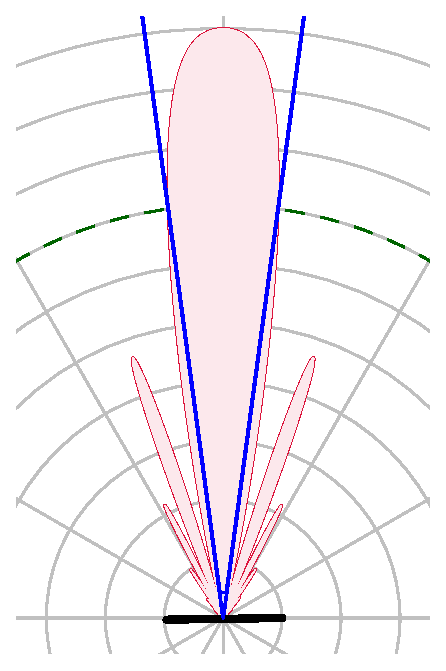
\includegraphics[scale=0.6,trim={0.46 0.072 0.46
	1.03},clip]{Chap2/fig/directivity.eps}
	\caption{Far field beam shape and its \textit{beamwidth} (in blue).}
	\label{fig:beamwidth}
\end{figure}

On the other hand, there are hydrophone arrays that can infer the sound
direction by relating the spacing between the transducers with the signal
difference received by each of them \cite{bearing,beamforming}. One technique is
very similar to \textit{multilateration}, simply compute the distance measured
by each transducer and use this information to compute the direction of the
incoming sound wave.

% figura bearing

Another possibility is to apply signal processing by delaying the received
signal from one hydrophone w.r.t. the other and adding them together. The
constructive/destructive interference effectively changes the directivity of the
array and, thus, can be used to find which direction gives the strongest echo.
This is known as \textit{beamforming}.

The sequence of transducers can be made into a two dimensional array
(a.k.a. a grid), making it possible to detect a full 3D direction.

\subsubsection{TVG - Time Varying Gain}\label{sss:tvg}

As sound waves propagates, they lose intensity through spreading and absorption.
Spreading loss is usually considered to be and inverse quadratic
law\cite{Etter2013}, as this is the closed surface area progression for
a time-like wavefront. But for cylindrical spreading it is a simple inverse law,
and for perfect plane wave there is no loss.

Absorption is conditional on the water characteristics and is modeled as a
slow exponential decay. Together with spreading, they are referred as
Transmission Loss ($\text{TL}$), in decibels (dB):

\begin{equation*}
\text{TL} = 20\log_{10}(r) + \alpha r
\end{equation*}

Where $r$ is the wave's total traveled distance and $\alpha$ a water dependent
parameter (with order of magnitude of $\approx 10^{-2} \text{dB}/m$). Sonars use
this equation, with a saturation around $40$dB, to compensate for the echo
loss\cite{chu2006time}. And, as distance is inferred from time measurements,
this compensative gain is named Time Varying Gain (TGV). \citet{chew2013object}
estimated TGV gain for a Tritech's Micron sonar and suggests that it agrees with
the expected.


\subsection{Available Models}
\label{ss:avaible_models}
 
Active Sonars, besides having a common working principle, present themselves in
different models for different applications. \citet{sonars:16} summarized the
most relevant ones.

\subsubsection{Mechanically Scanning}

As seen on subsection \ref{sss:bearing}, it is possible to use the beam shape as
a way to reduce the number of possible incoming directions for an echo. This is
the idea behind a mechanically scanning sonar, where the transducer is
mechanically rotated to cover all or part of the $360^o$.

The angular step between different hydrophone's positions is dependent on the
desired resolution, smaller steps gives a better resolution, but takes longer
by doing so.

\begin{enumerate}
  \item \textbf{Profiling} - possessing a narrow conical beam shape, they are the
  acoustic analog of a laser scanner (although they still have a much larger
  aperture than a laser). Only a single echo is recorded for each angular
  position, either the strongest or the first to return. Typically, applied for
  pipeline surveillance, they can spot structural differences and objects on
  sea floor.
  \item \textbf{Imaging} - its fan shaped narrow beam covers a wider area than
  the profiling type, making it very useful for navigation and obstacle
  avoidance on ROVs\footnote{Remotely Operated underwater Vehicle}. As its beam
  is wide, it usually hits the surface obliquely, receiving several echos per
  acoustic pulse. Each echo is displayed at a distance determined by equation
  \ref{eq:delaytodistance} and with its strength mapped to a color scale.
  \item \textbf{Side Scan} (a.k.a. towfish) - Can be either mounted on each side
      %% SrJ?: not sure about the beam shape, for the sidescan is usually more
      % of
      %% SrJ: profiler
  of a boat's hull or towed behind. Usually with a beam shape similar to an
  imaging sonar, it can provide a sophisticated image of the sea floor.
  \item \textbf{Echo-sounder} - mounted below a boat, it has a narrow pulse
  (as a profiling) with the single purpose of measuring the depth of water. It
  is typically applied to help with navigation or constructing depths charts.
\end{enumerate}

% profiling / imaging sonar

\subsubsection{Multibeam}

Multibeam sonar are based on the technique of \textit{beamforming} (described
on section \ref{sss:bearing}). It has several hydrophones, rendering it able to
scan an underwater region with no moving parts.

%% SrJ: actually, in the multibeam world, the only difference between profiling
%% SrJ: imaging is the beam height. The data is presented in exactly the same
% way
%%
%% SrJ: the thing is, profilers are more sensitive to errors in the measurement
%% SrJ: and processing, so are harder to make

\begin{enumerate}
  \item \textbf{Profiling} - similar in application to its mechanically scanning
  counterpart, it has multiple narrow conical beam receivers that record the
  signal. Instead of moving its transducer, it amplifies and processes (through
  \textit{beamforming}) the received signal to identify the position of the
  strongest returned echo, then creating a high-speed cross-sectional profile.
  \item \textbf{Imaging} - it is much quicker than a Mechanical Imaging
  %% SrJ: "crispier image" is more an effect of generation than technique
  Sonar, being very similar to a Multibeam Profiling their difference lies on
  beamwidth.   It possesses a wide angle acoustic transmitter and multiple
  narrow beam receivers, applying \textit{beamforming} to the received signal.
\end{enumerate}

The array size of hydrophones is critical for enhancing resolution, longer
arrays have a better angular resolution. To overcome physical limitations a
technique known as \textit{SAS} (Synthetic Aperture Sonar) may be applied. The
transmission of several acoustic pulses in a line is used to emulate the
presence of a longer array, by means of signal processing on the reception.
